% !TeX root = main.tex

\subsection{Collision cone based constant time-scaling}

A collision cone is comprised of the relative velocities of the robot (with reference to an obstacle) that will lead to a collision in the future. Usually, we assume a linear velocity trajectory (for both robot and obstacle). However, the method can be generalized to any \emph{robot} profile (say a bernstein profile) using an iterative approach (as we do ahead).

\begin{figure}[ht]
    \begin{subfigure}[b]{0.24\textwidth}
        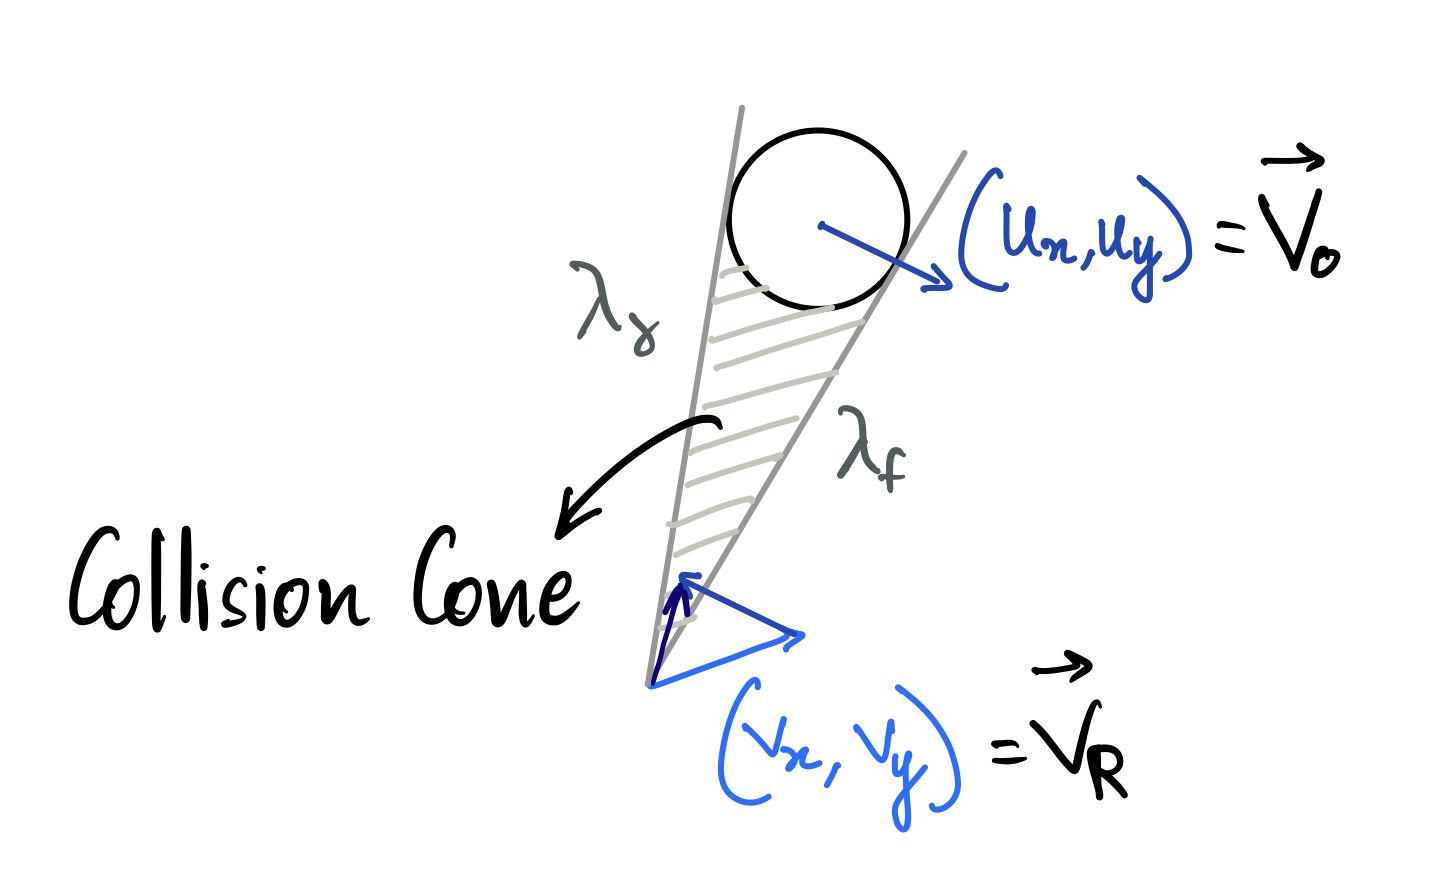
\includegraphics[width=\textwidth]{cc-img1.PNG}
        \caption{Collision Cone}
        \label{fig:sfig-cc-cts}
    \end{subfigure}
    \begin{subfigure}[b]{0.24\textwidth}
        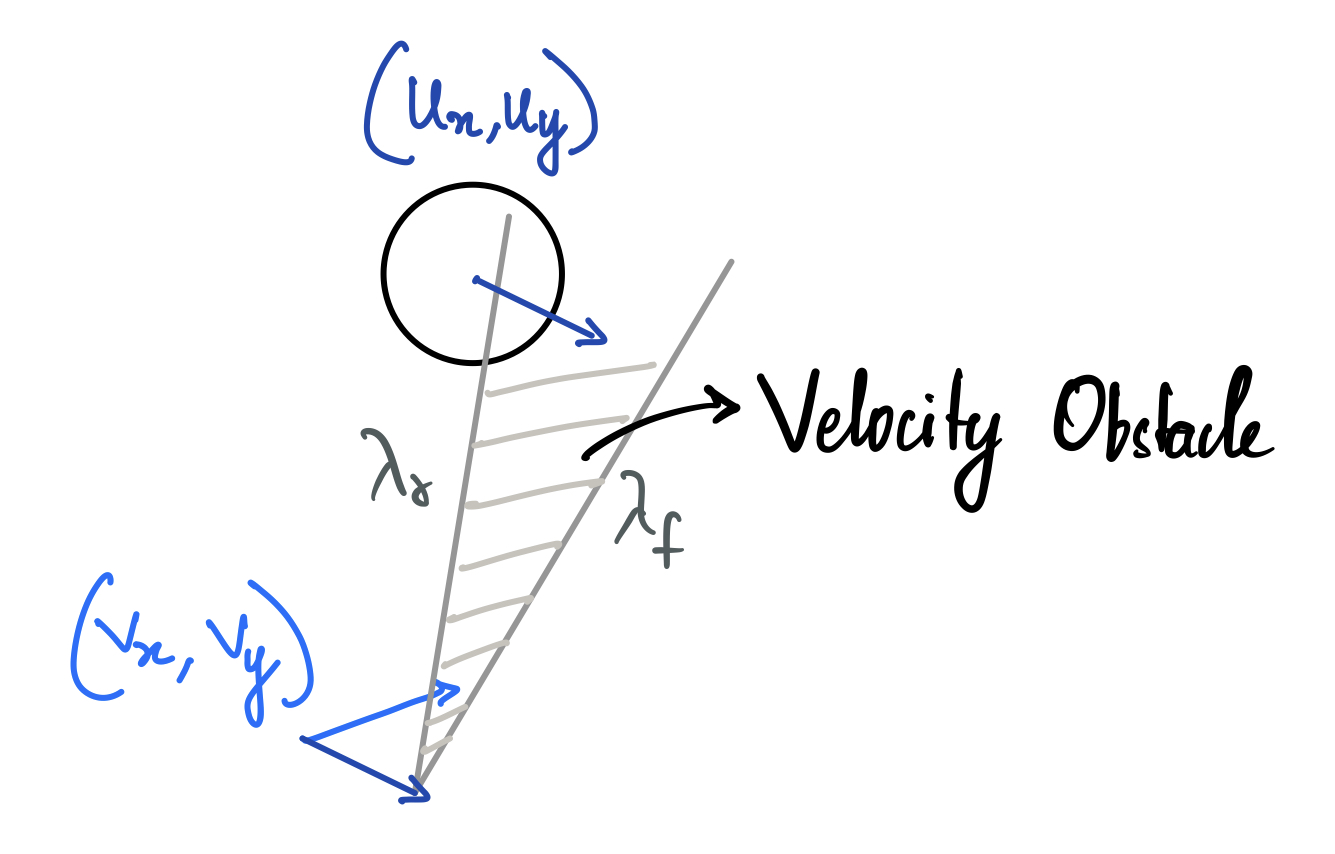
\includegraphics[width=\textwidth]{cc-img2.PNG}
        \caption{Velocity Obstacle}
        \label{fig:sfig-vo-cts}
    \end{subfigure}
    \begin{subfigure}[b]{0.24\textwidth}
        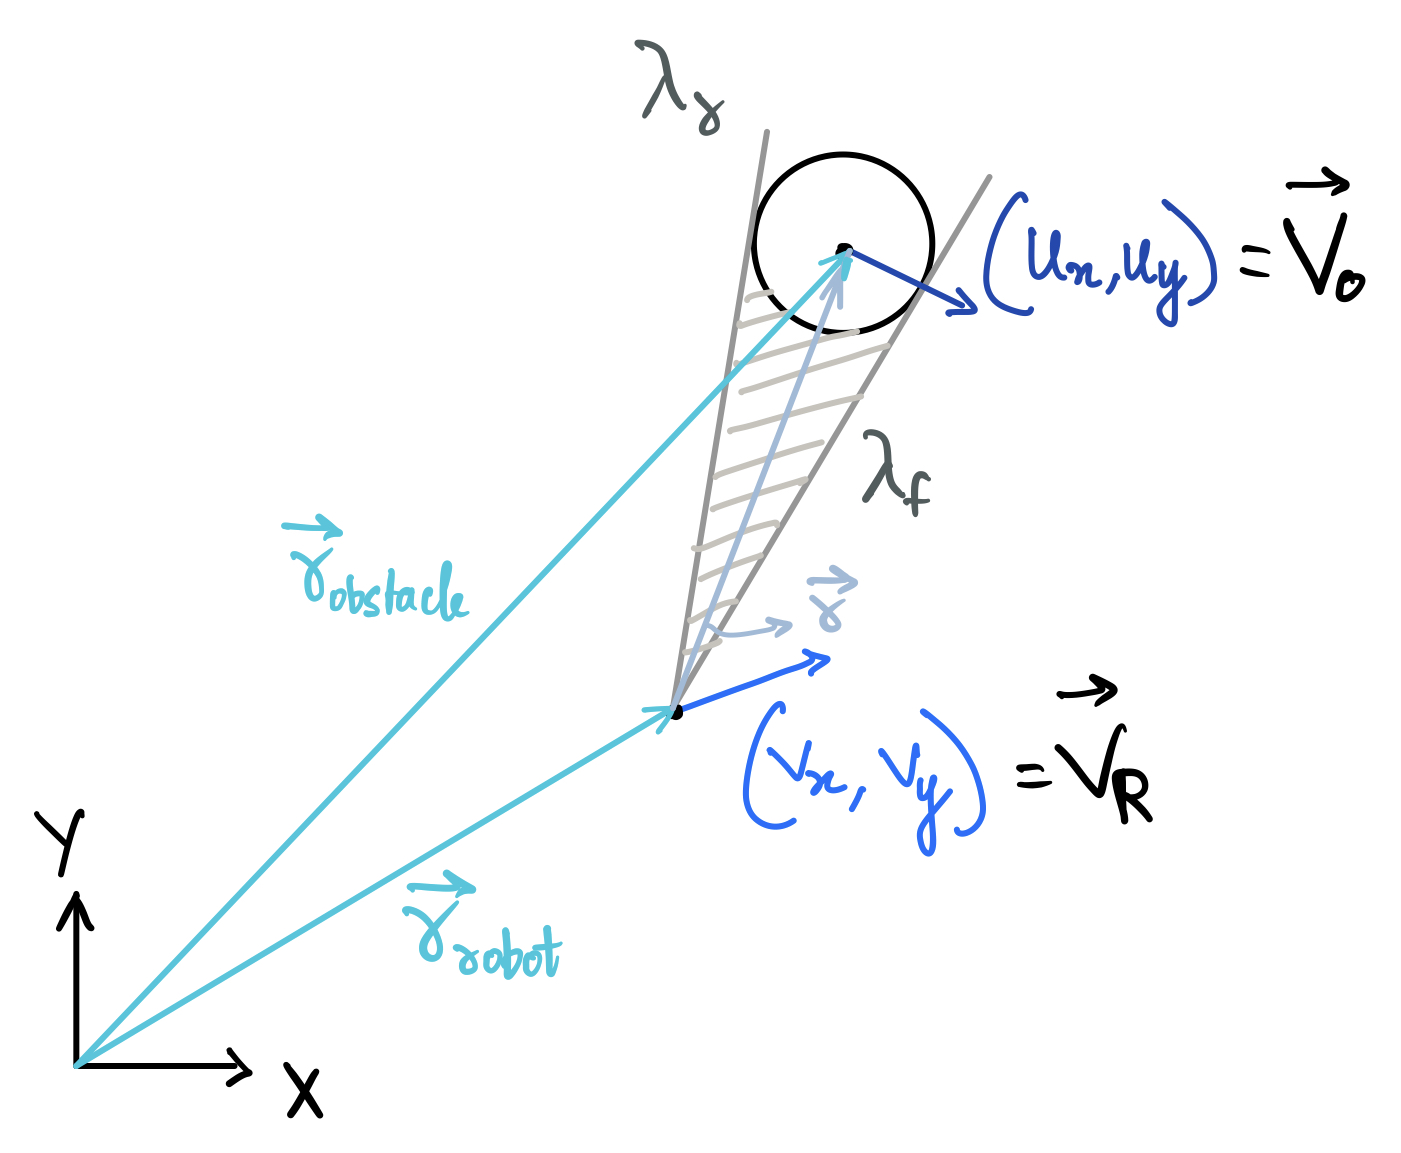
\includegraphics[width=\textwidth]{cc-img3.PNG}
        \caption{Environment}
        \label{fig:sfig-env-cts}
    \end{subfigure}
    \begin{subfigure}[b]{0.24\textwidth}
        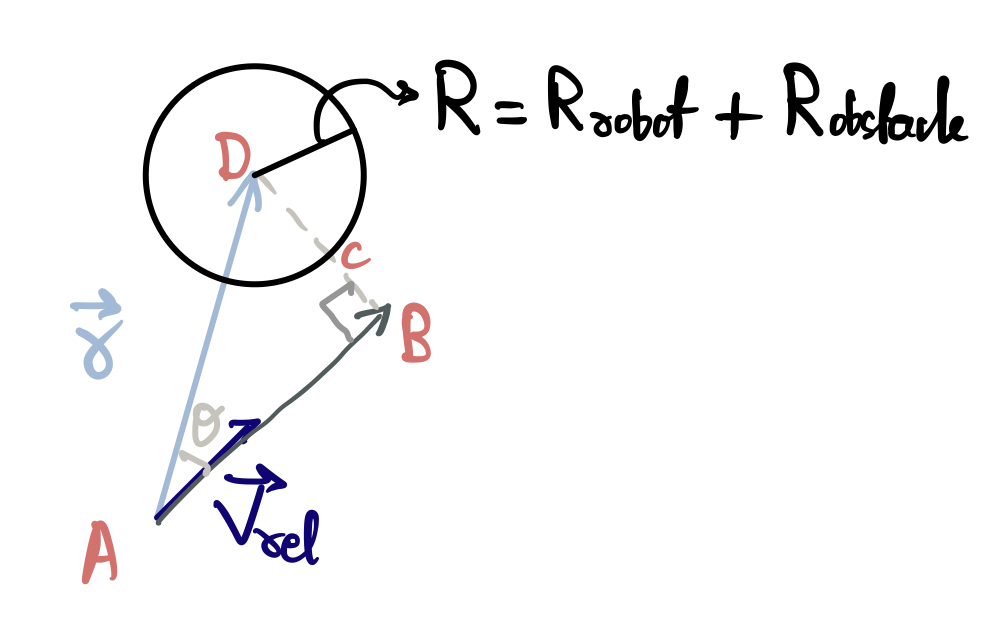
\includegraphics[width=\textwidth]{cc-img4.PNG}
        \caption{Avoiding collision}
        \label{fig:sfig-ac-cts}
    \end{subfigure}
    \caption{Collision Cone}
    \label{fig:cc-cts-imgs}
    \small
        The velocity of obstacle is $\overrightarrow{V}_{O} = (u_x, u_y)$. The velocity of obstacle is $\overrightarrow{V}_{R} = (v_x, v_y)$. THe radius of robot is $R_{robot}$ and the radius of obstacle is $R_{obstacle}$. The obstacle is diluted to $R = R_{robot} + R_{obstacle}$ while the robot is reduced to a point.

        After time scaling, the velocity of the robot becomes scaled by a factor of $s$, that is, the time scaled robot velocity is $\vec{V}_{R} = (s\dot{x}_1, s\dot{y}_1)$.
\end{figure}

The collision cone is shown in figure \ref{fig:sfig-cc-cts}. The \emph{velocity obstacle} is obtained by adding the obstacle velocity vector to the collision cone (as shown in figure \ref{fig:sfig-vo-cts}). The robot's velocity should be out of the velocity obstacle.

Consider the environment with the collision cone (as in figure \ref{fig:sfig-env-cts}). By looking into a zoomed version of it (as in figure \ref{fig:sfig-ac-cts} - use this for variables in the equations), we can formulate the following to avoid a collision

\begin{align*}
    \textup{DB} \ge \textup{DC} \Rightarrow
    \textup{DB}^2 \ge R^2 \Rightarrow
    \textup{AD}^2 - \textup{AB}^2 \ge R^2
    &&
    \vec{r}_{obstacle} = \vec{r}_{robot} + \vec{r} \Rightarrow 
    \vec{r} = \vec{r}_{obstacle} - \vec{r}_{robot}
    \\
    \textup{AB} = \left \| \vec{r} \right \| \cos(\theta) = \frac{\vec{V}_{rel} \cdot \vec{r}}{\left \| \vec{V}_{rel} \right \|}
    \Rightarrow \textup{AB}^2 = \left [ \frac{\vec{V}_{rel} \cdot \vec{r}}{\left \| \vec{V}_{rel} \right \|} \right ]^2
    &&
    \textup{AD} = \left \| \vec{r} \right \| \Rightarrow \textup{AD}^2 = \left \| \vec{r} \right \|^2
\end{align*}

\begin{align*}
    \vec{V}_{rel} = \vec{V}_{R} - \vec{V}_{O} = (s\dot{x}_1 - \dot{x}_2, s\dot{y}_1 - \dot{y}_2)
    &&
    \vec{r} = \vec{r}_{obstacle} - \vec{r}_{robot} = (x_2 - x_1, y_2 - y_1) \\
    \textup{AD}^2 - \textup{AB}^2 \ge R^2 \Rightarrow 
    \left \| \vec{r} \right \|^2 - \left [ \frac{\vec{V}_{rel} \cdot \vec{r}}{\left \| \vec{V}_{rel} \right \|} \right ]^2 \ge R^2
    &&
    \left \| \vec{r} \right \|^2 - \left [ \frac{\vec{V}_{rel} \cdot \vec{r}}{\left \| \vec{V}_{rel} \right \|} \right ]^2 - R^2 \ge 0
    \\
    \vec{V}_{rel} \cdot \vec{r} = (s\dot{x}_1 - \dot{x}_2) (x_2 - x_1) + (s\dot{y}_1 - \dot{y}_2) (y_2 - y_1)
    &&
    \left \| \vec{V}_{rel} \right \| = \sqrt{\left( s\dot{x}_1 - \dot{x}_2 \right)^2 + \left( s\dot{y}_1 - \dot{y}_2 \right)^2}
\end{align*}

\begin{align}
    (x_1 - x_2)^2 + (y_1 - y_2)^2 - R^2 - \frac{\left( (s\dot{x}_1 - \dot{x}_2) (x_2 - x_1) + (s\dot{y}_1 - \dot{y}_2) (y_2 - y_1) \right)^2}{\left( s\dot{x}_1 - \dot{x}_2 \right)^2 + \left( s\dot{y}_1 - \dot{y}_2 \right)^2} \ge 0
    \label{eq:cc-cts-rawineq}
\end{align}

We represent equation \ref{eq:cc-cts-rawineq} in the form $a s^2 + b s + c \ge 0$. This gives us the following solution space (set) for $s$

\begin{equation}
    S_{sol} = \left\{\begin{matrix}
        [s_{min}, \infty) \cap \left ( (-\infty, \gamma_1] \cup [\gamma_2, \infty) \right ) && a > 0,\, d > 0 \\
        [s_{min}, \infty) && a > 0,\, d < 0 \\
        [s_{min}, \infty) \cap [\gamma_1, \gamma_2] && a < 0 ,\, d > 0 \\
        \phi && a < 0 ,\, d < 0
    \end{matrix}\right.
    \label{eq:cc-cts-solspace-s}
\end{equation}

Where

\begin{align*}
    d = b^2 - 4ac
    &&
    \gamma_1 = \frac{-b - \sqrt{d}}{2a}
    &&
    \gamma_2 = \frac{-b + \sqrt{d}}{2a}
\end{align*}

And $s_{min} = 0.1$ (minimum scaling factor). We pick $s = \min\{S_{sol}\}$ (minimum of the solution space).

Usually, equation \ref{eq:cc-cts-solspace-s} is accompanied with acceleration constraints of the vehicle. The code for this experiment uses \texttt{sympy} to find this quadratic equation's coefficients $a$, $b$, and $c$. The code is available in appendix \ref{app:nh-cc-cts-code}.

The graphs for the runs are shown in figure \ref{fig:cc-cts-exp1-graphs}, and snaps from the simulation are shown in figure \ref{fig:cc-cts-exp1}. You can see that here, extra time is not wasted after avoiding collision (thanks to automatic sensing of distances and choice of the scaling factor).

\begin{figure}
    \centering
    \begin{subfigure}[b]{0.49\textwidth}
        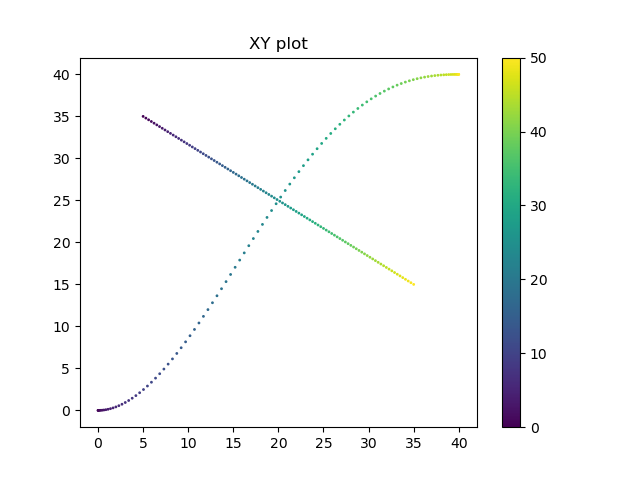
\includegraphics[width=\textwidth]{cc-cts-xy-plot.png}
        \caption{XY plots}
        \label{fig:sfig-cc-cts-e1-xy}
        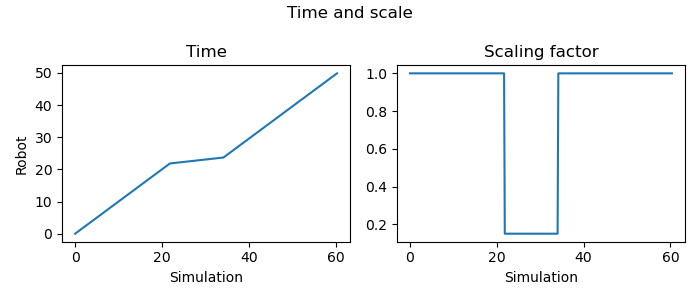
\includegraphics[width=\textwidth]{cc-cts-timescales.png}
        \caption{Time scaling}
        \label{fig:sfig-cc-cts-e1-ts}
    \end{subfigure}
    \begin{subfigure}[b]{0.49\textwidth}
        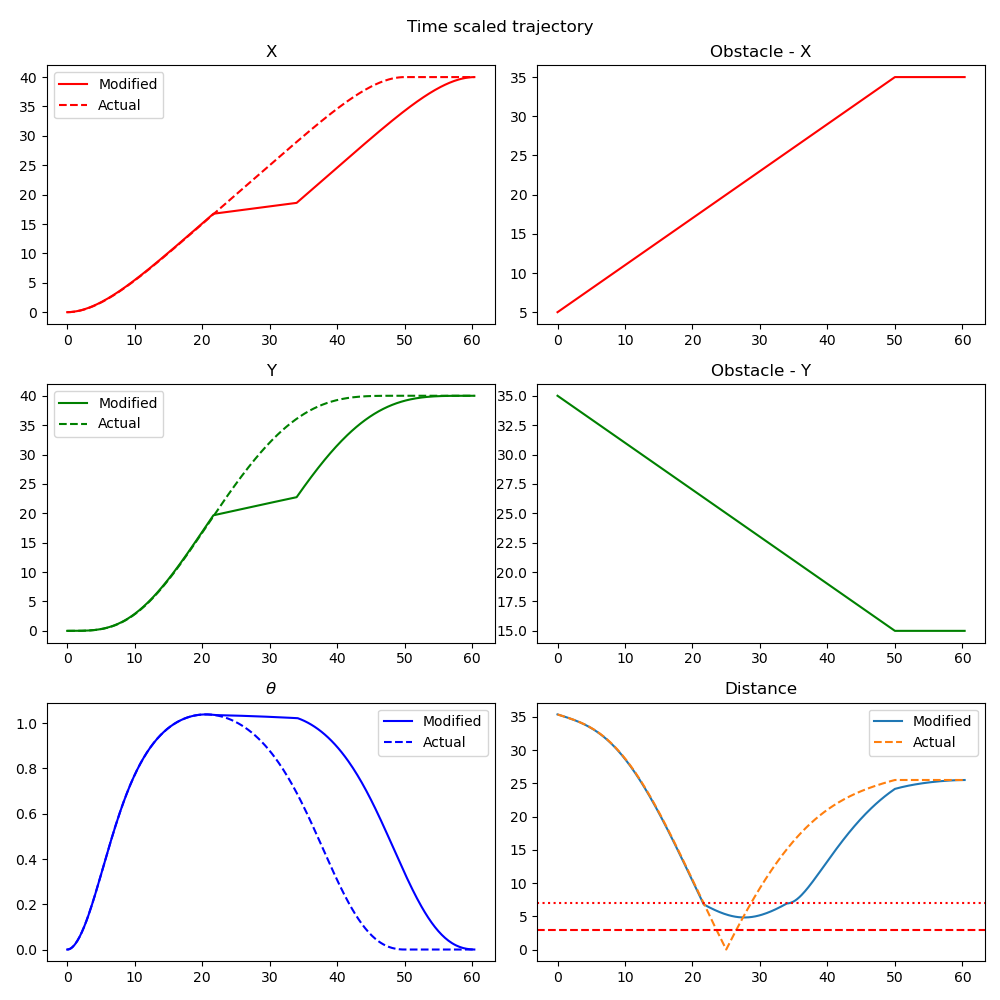
\includegraphics[width=\textwidth]{cc-cts-trajs.png}
        \caption{Time scaled results}
        \label{fig:sfig-cc-cts-e1-fgr}
    \end{subfigure}
    \caption{Collision cone based constant time scaling}
    \label{fig:cc-cts-exp1-graphs}
    \small
        The distance plot is shown in the bottom right of \ref{sub@fig:sfig-cc-cts-e1-fgr}. As seen, the time scaling gets activated at the thin red horizontal line (detection distance) and a collision is avoided (the distance plot does not cross the thick horizontal red line). See the slope and the scaling factor change in \ref{sub@fig:sfig-cc-cts-e1-ts}. The original (colliding) trajectories are shown in \ref{sub@fig:sfig-cc-cts-e1-xy}.
\end{figure}

\begin{figure}
    \centering
    \begin{subfigure}[b]{0.3\textwidth}
        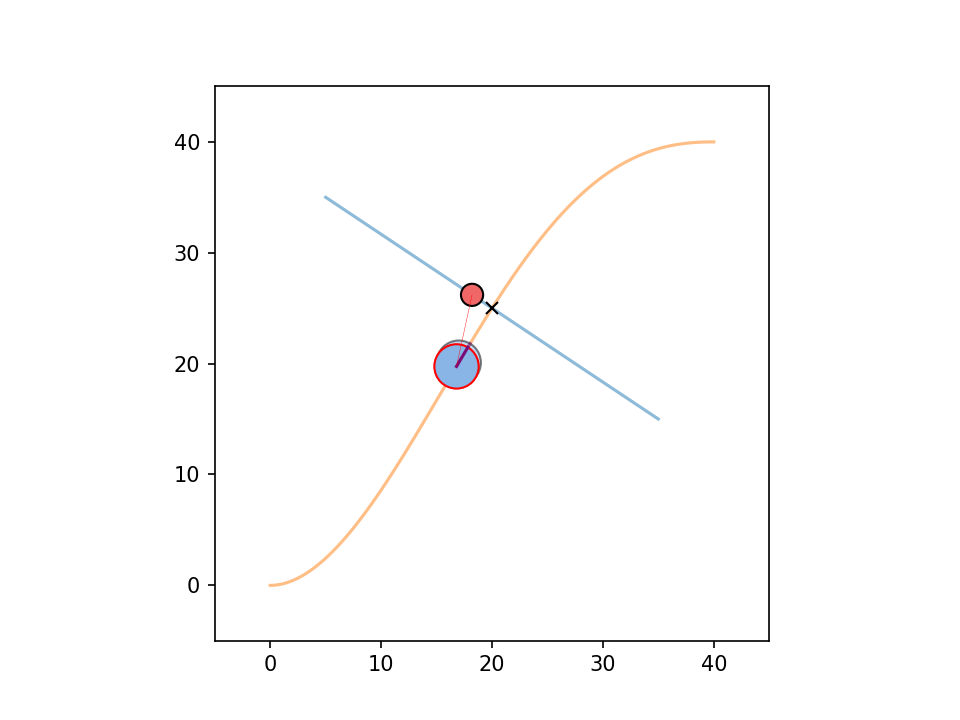
\includegraphics[width=\textwidth]{res2-ts-start.png}
        \caption{Start}
    \end{subfigure}
    \begin{subfigure}[b]{0.3\textwidth}
        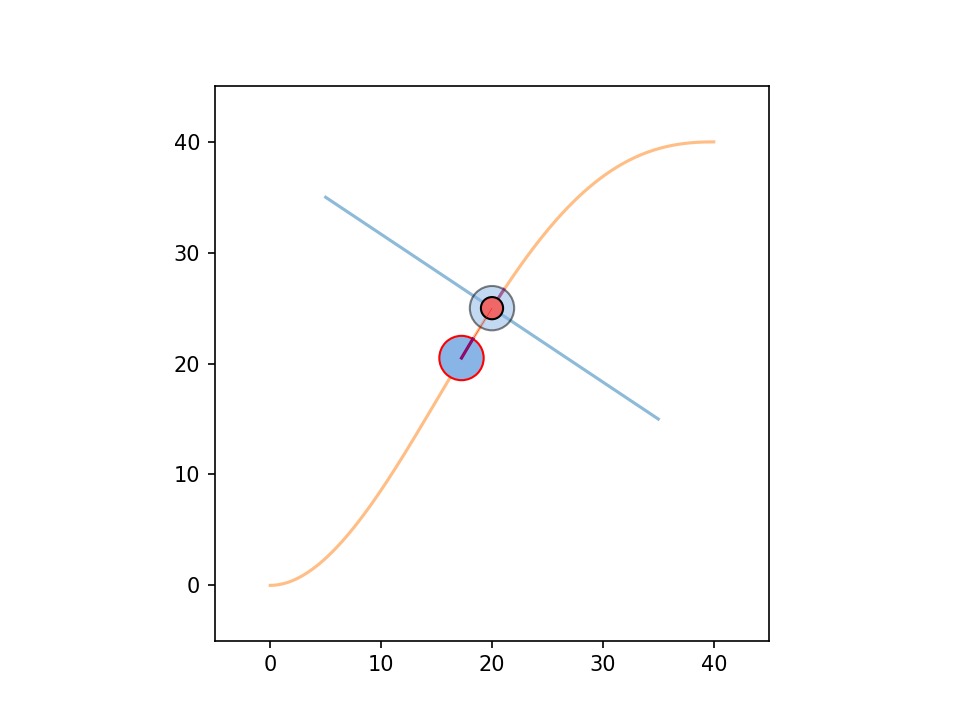
\includegraphics[width=\textwidth]{res2-ts-colav.png}
        \caption{Collision avoidance}
    \end{subfigure}
    \begin{subfigure}[b]{0.3\textwidth}
        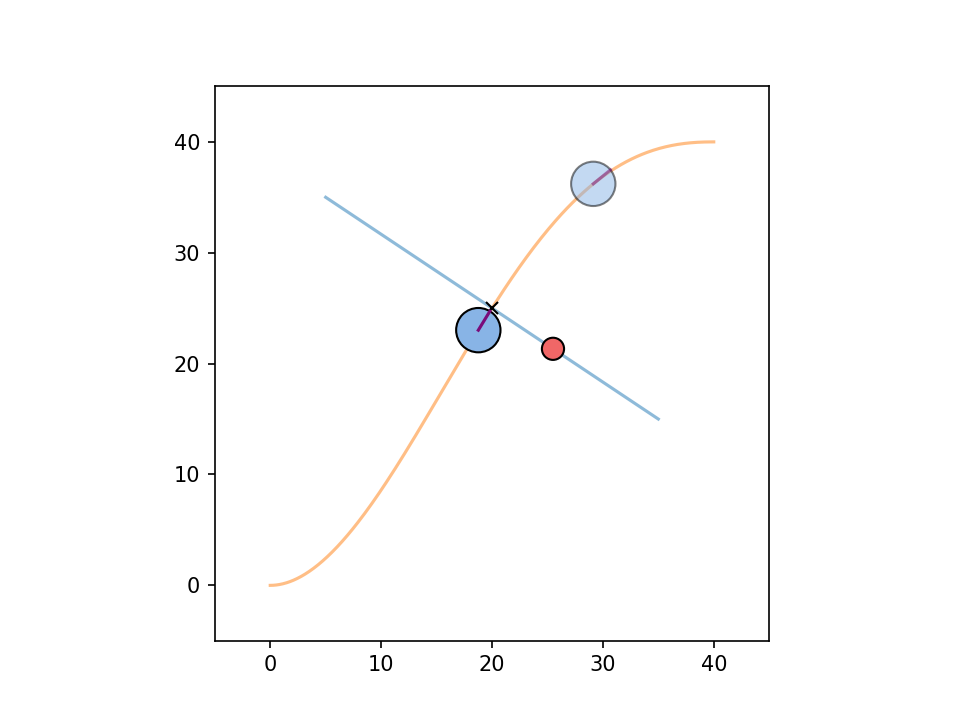
\includegraphics[width=\textwidth]{res2-ts-end.png}
        \caption{End}
    \end{subfigure}
    \caption{Collision cone - Constant time scaling - Video snaps}
    \label{fig:cc-cts-exp1}
    \small
        The simulation is available as \texttt{cc\_cts\_exp1.avi} in the \href{https://iiitaphyd-my.sharepoint.com/:f:/g/personal/avneesh_mishra_research_iiit_ac_in/Er_wRqK4hxVLjVdL56rfDxYBKr9PPed1laN48hLgLisf4w}{shared OneDrive folder}. The time scaling turns off here when the obstacle passes, unlike in figure \ref{fig:rb-cts-exp1} (where everything is hardcoded).

        Another experiment is present as \texttt{cc\_cts\_exp2.avi} in the same shared folder.
\end{figure}
